\documentclass[tikz,border=12pt]{standalone}
\usepackage[T1]{fontenc}
\usepackage{mathpazo}
\usepackage{amsmath,amssymb}
\usetikzlibrary{arrows.meta, positioning, calc, fit, decorations.pathreplacing}

\definecolor{stblue}{HTML}{7B97AD}
\definecolor{rwgold}{HTML}{B8995E}
\definecolor{sage}{HTML}{7A9A7E}
\definecolor{dkbrown}{HTML}{3D3530}
\definecolor{wmgray}{HTML}{7B7067}
\definecolor{cream}{HTML}{F9F6F0}
\definecolor{border}{HTML}{D4C9B8}
\definecolor{terracotta}{HTML}{C47A6A}

\begin{document}
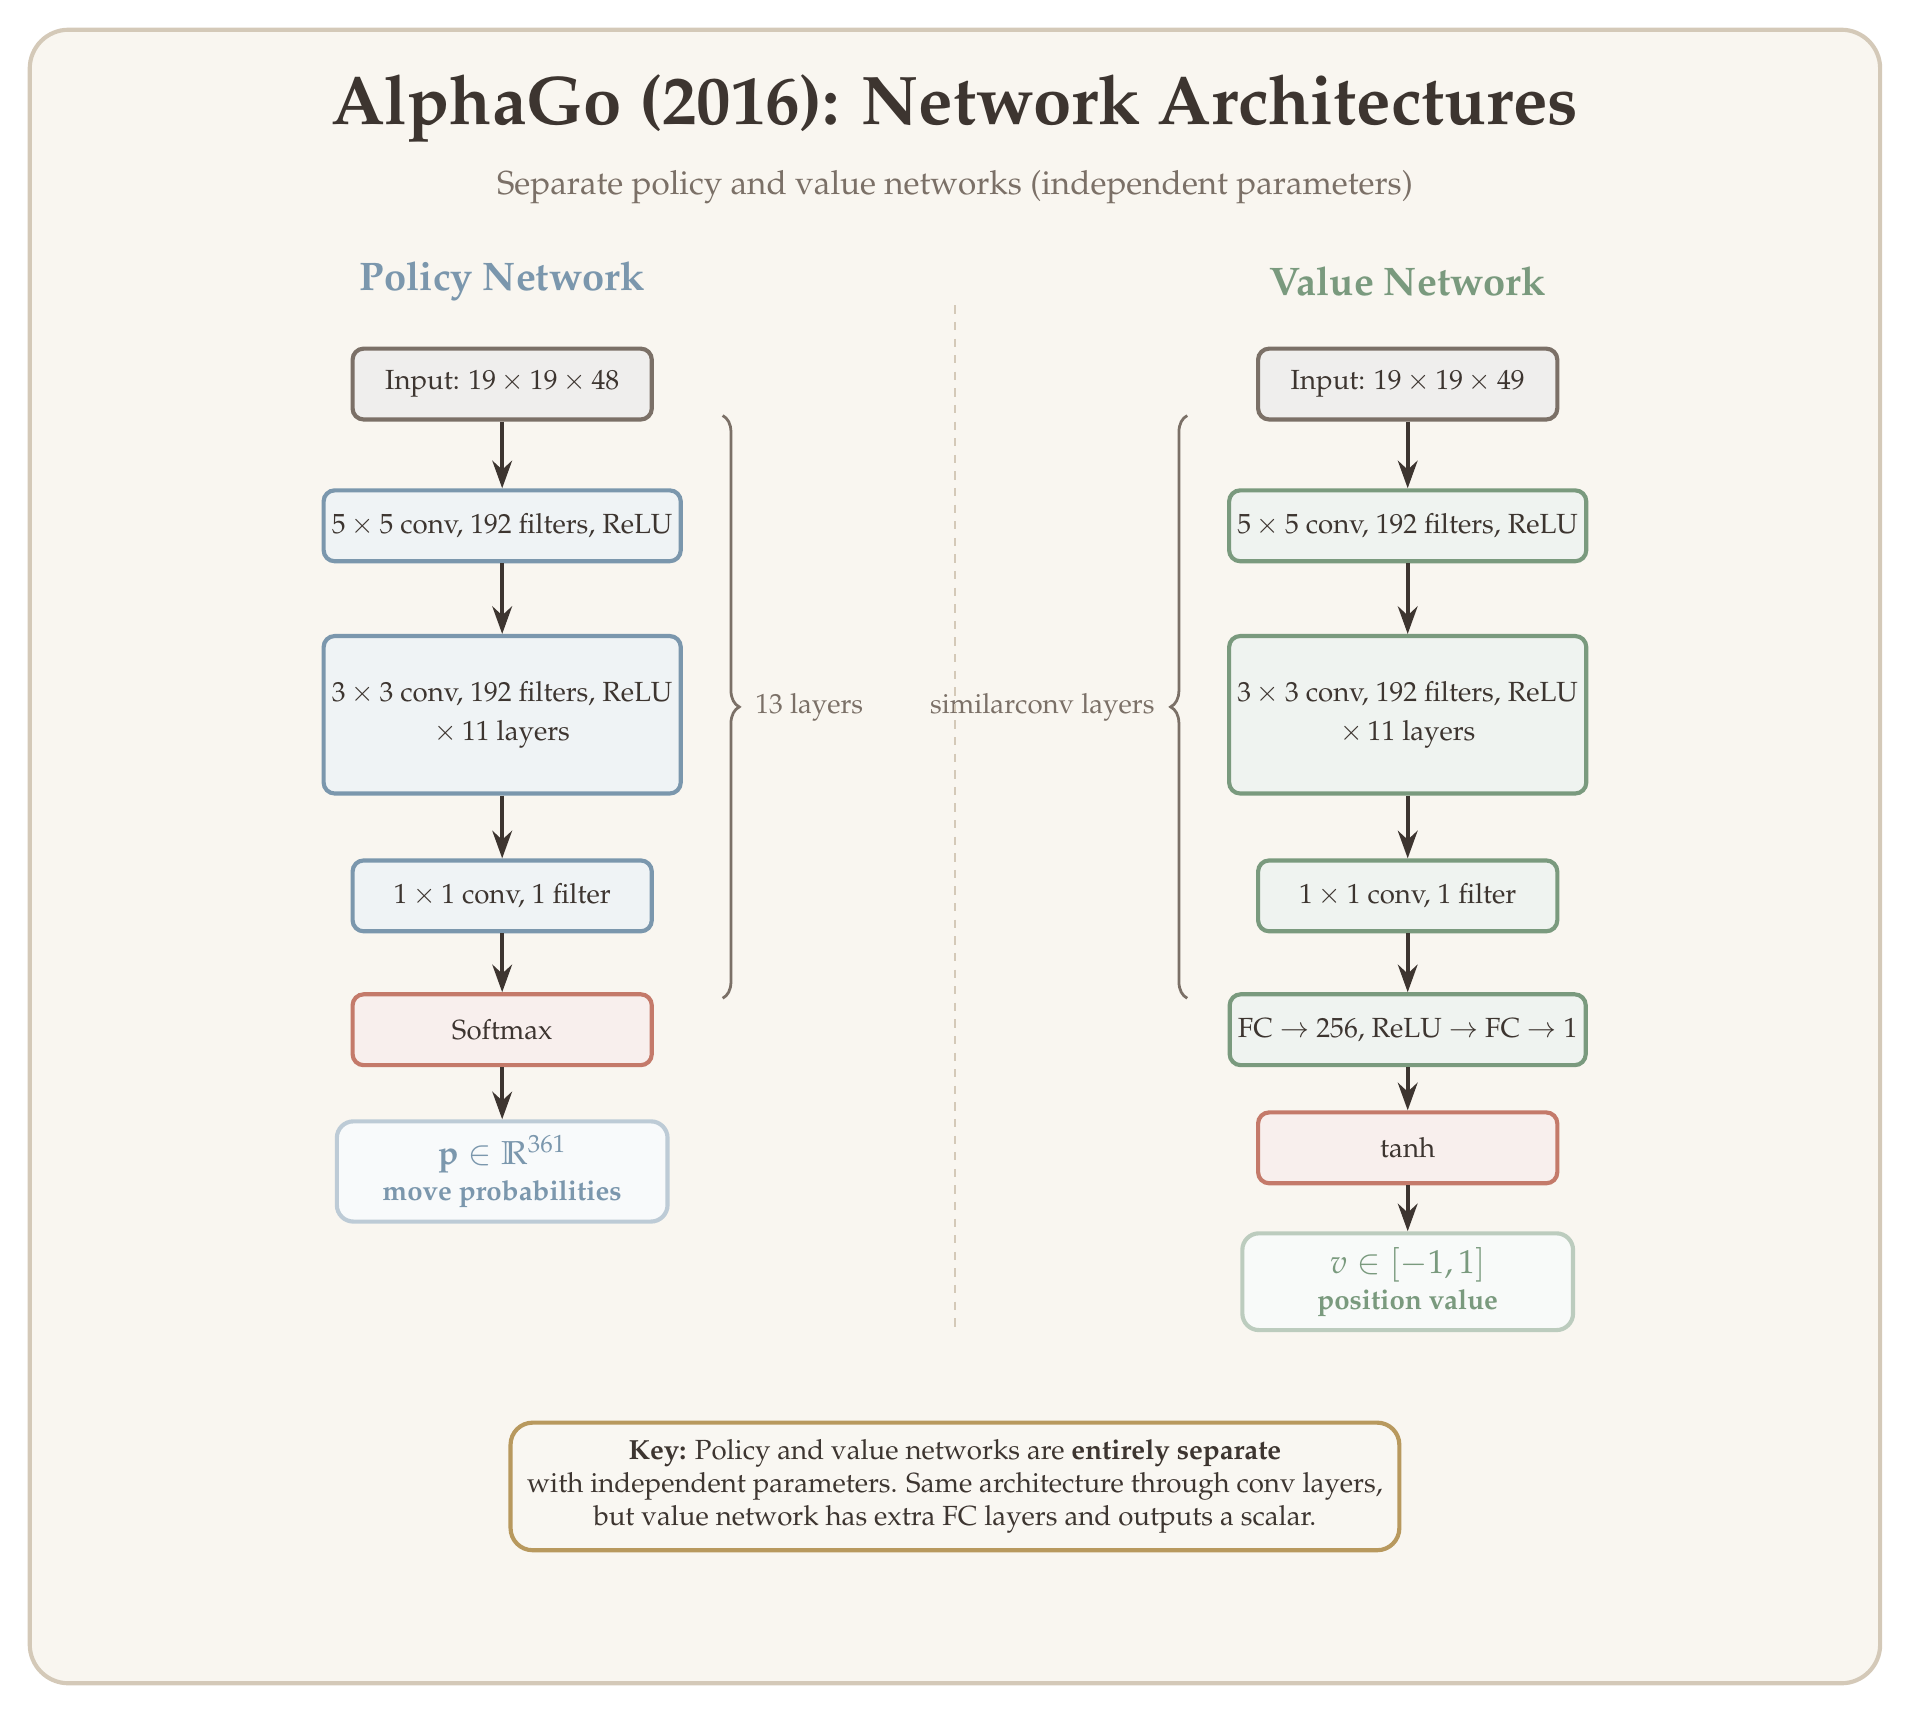
\begin{tikzpicture}[
  >={Stealth[length=3.5mm, width=2.5mm]},
  layer/.style={
    draw=#1, line width=1.5pt, fill=#1!12, rounded corners=4pt,
    minimum width=38mm, minimum height=9mm, font=\normalsize, text=dkbrown,
    align=center, inner sep=3pt
  },
  arr/.style={->, line width=1.5pt, dkbrown},
  lbl/.style={font=\normalsize, text=wmgray, align=center},
]

% Background
\fill[cream, rounded corners=14pt] (-2,-1.5) rectangle (21.5,19.5);
\draw[border, rounded corners=14pt, line width=1.5pt] (-2,-1.5) rectangle (21.5,19.5);

% Title
\node[font=\Huge\bfseries, text=dkbrown] at (9.75,18.5)
  {AlphaGo (2016): Network Architectures};

% Subtitle
\node[font=\large, text=wmgray] at (9.75,17.5)
  {Separate policy and value networks (independent parameters)};

% =============================================
% LEFT: Policy Network
% =============================================
\node[font=\Large\bfseries, text=stblue] at (4,16.3) {Policy Network};

% Input
\node[layer=wmgray] (pi-in) at (4,15)
  {Input: $19 \times 19 \times 48$};

% Conv 1
\node[layer=stblue] (pi-c1) at (4,13.2)
  {$5 \times 5$ conv, 192 filters, ReLU};

% Conv 2-12
\node[layer=stblue, minimum height=20mm] (pi-c2) at (4,10.8)
  {$3 \times 3$ conv, 192 filters, ReLU\\[2pt]
   $\times\, 11$ layers};

% Conv 13
\node[layer=stblue] (pi-c3) at (4,8.5)
  {$1 \times 1$ conv, 1 filter};

% Softmax
\node[layer=terracotta] (pi-out) at (4,6.8)
  {Softmax};

% Output
\node[draw=stblue!50, line width=1.5pt, fill=stblue!5, rounded corners=6pt,
      minimum width=42mm, minimum height=12mm, font=\large\bfseries, text=stblue,
      align=center, inner sep=5pt]
  (pi-result) at (4,5)
  {$\mathbf{p} \in \mathbb{R}^{361}$\\[-1pt]
   {\normalsize move probabilities}};

% Arrows
\draw[arr] (pi-in) -- (pi-c1);
\draw[arr] (pi-c1) -- (pi-c2);
\draw[arr] (pi-c2) -- (pi-c3);
\draw[arr] (pi-c3) -- (pi-out);
\draw[arr] (pi-out) -- (pi-result);

% Brace for 13 layers
\draw[decorate, decoration={brace, amplitude=6pt}, line width=1pt, wmgray]
  (6.8,14.6) -- (6.8,7.2) node[midway, right, xshift=8pt, font=\normalsize, text=wmgray]
  {13 layers};

% =============================================
% RIGHT: Value Network
% =============================================
\node[font=\Large\bfseries, text=sage] at (15.5,16.3) {Value Network};

% Input
\node[layer=wmgray] (v-in) at (15.5,15)
  {Input: $19 \times 19 \times 49$};

% Conv 1
\node[layer=sage] (v-c1) at (15.5,13.2)
  {$5 \times 5$ conv, 192 filters, ReLU};

% Conv 2-12
\node[layer=sage, minimum height=20mm] (v-c2) at (15.5,10.8)
  {$3 \times 3$ conv, 192 filters, ReLU\\[2pt]
   $\times\, 11$ layers};

% Conv 13
\node[layer=sage] (v-c3) at (15.5,8.5)
  {$1 \times 1$ conv, 1 filter};

% FC
\node[layer=sage] (v-fc) at (15.5,6.8)
  {FC $\to$ 256, ReLU $\to$ FC $\to$ 1};

% Tanh
\node[layer=terracotta] (v-tanh) at (15.5,5.3)
  {$\tanh$};

% Output
\node[draw=sage!50, line width=1.5pt, fill=sage!5, rounded corners=6pt,
      minimum width=42mm, minimum height=12mm, font=\large\bfseries, text=sage,
      align=center, inner sep=5pt]
  (v-result) at (15.5,3.6)
  {$v \in [-1, 1]$\\[-1pt]
   {\normalsize position value}};

% Arrows
\draw[arr] (v-in) -- (v-c1);
\draw[arr] (v-c1) -- (v-c2);
\draw[arr] (v-c2) -- (v-c3);
\draw[arr] (v-c3) -- (v-fc);
\draw[arr] (v-fc) -- (v-tanh);
\draw[arr] (v-tanh) -- (v-result);

% Brace
\draw[decorate, decoration={brace, amplitude=6pt, mirror}, line width=1pt, wmgray]
  (12.7,14.6) -- (12.7,7.2) node[midway, left, xshift=-8pt, font=\normalsize, text=wmgray]
  {similar\\conv layers};

% =============================================
% Center annotation: separate networks
% =============================================
\node[draw=rwgold, line width=1.5pt, fill=rwgold!8, rounded corners=8pt,
      font=\normalsize, text=dkbrown, align=center, inner sep=6pt]
  at (9.75,1)
  {\textbf{Key:} Policy and value networks are \textbf{entirely separate}\\
   with independent parameters. Same architecture through conv layers,\\
   but value network has extra FC layers and outputs a scalar.};

% Dividing line
\draw[border, line width=1pt, dashed] (9.75,16) -- (9.75,3);

\end{tikzpicture}
\end{document}
